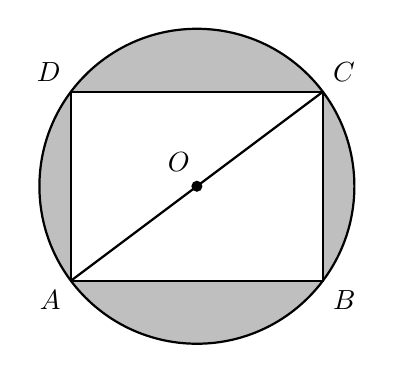
\begin{tikzpicture}[thick]
% Define dimensions
\def\r{2}      % circle radius
\def\a{1.6}    % rectangle half-width
\def\b{1.2}    % rectangle half-height  (a^2 + b^2 = r^2)

% Fill circular segments with solid grey (circle minus rectangle)
\fill[gray!50] (0,0) circle (\r);
\fill[white] (-\a,-\b) rectangle (\a,\b);

% Draw circle
\draw (0,0) circle (\r);

% Draw rectangle
\draw (-\a,-\b) rectangle (\a,\b);

% Draw diagonals (visible in the figure)
\draw (-\a,-\b) -- (\a,\b);

% Center point O
\fill (0,0) circle (2pt);
\node[above right] at (-0.5,0.05) {$O$};

% Labels
\node[below left]  at (-\a,-\b) {$A$};
\node[below right] at (\a,-\b)  {$B$};
\node[above right] at (\a,\b)   {$C$};
\node[above left]  at (-\a,\b)  {$D$};

\end{tikzpicture}